\documentclass{IEEEtran}

\usepackage{amssymb}
\usepackage{graphicx}
\usepackage{caption}
\usepackage{subcaption}
\usepackage[colorlinks,linkcolor=blue]{hyperref}
\usepackage{todonotes}

\begin{document}
    \title{\textbf{TransportIDE} -- An integrated transportation system design and simulation environment}
    \author{Dominik Ascher and Georg Hackenberg}
    \maketitle
    
    \begin{abstract}
        Due to many reasons transportation systems have to become more and more efficient.
        This observation holds true both for person transport and for good transport, on public infrastructure and on private infrastructure.
        Designing efficient transportation systems is a difficult undertaking due to the vast size of the solution space and the emergent dynamics of the system components.
        Transportation system designers need appropriate tools to explore the design space and test solutions quickly and reliably.
        In this paper, we propose a simulation-based environment for transportation system design and test, which is built on a solid system theory.
        Furthermore, we demonstrate possible applications such as comparison of different infrastructure and control algorithm designs.
    \end{abstract}
    
    \section{Introduction}
    \label{sec:intro}
    TODO

    \newpage

    \subsection{Research question}
    How can we support the design and test of transportation infrastructures and control algorithms better?
    Which modeling and simulation technique represents an appropriate abstraction for the domain?
    Which software architecture is appropriate for an integrated design and test environment?
    Which application scenarios should be supported on top of this environment?

    \subsection{Research methodology}
    To answer the above questions, we apply and combine two research methodologies.
    First we conduct a literature review to understand the state of the art in transportation system design and test.
    Second we use iterative and incremental software development with regular feedback from stakeholders to develop our a new dedicated approach.

    \subsection{Document outline}
    In the following, w e first present related work on transportation system design and test in Section~\ref{sec:related}.
    Then we describe the underlying system theory of our approach in Section~\ref{sec:theory}.
    Afterwards, we explain our software architecture in Section~\ref{sec:arch}.
    Thereafter, we demonstrate three software applications in Section~\ref{sec:app}.
    Finally, we draw our conclusion in Section~\ref{sec:con}.
    
    \begin{figure*}[t]
        \centering
        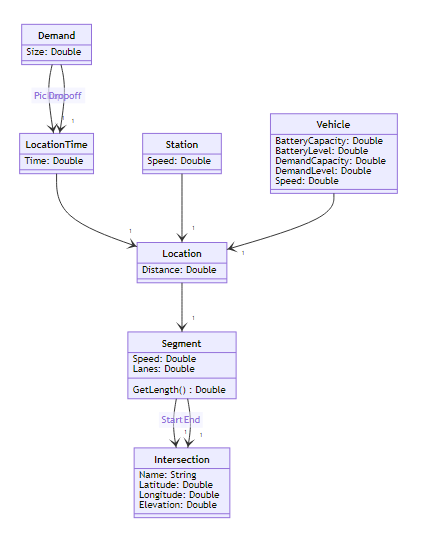
\includegraphics[scale=0.5]{../../diagrams/model/classes-v0.png}
        \caption{Concepts in UML class diagram notation}
        \label{fig:concepts}
    \end{figure*}

    \newpage

    \section{Related work}
    \label{sec:related}
    TODO

    \newpage

    \section{System theory}
    
    \label{sec:theory}
    In the following, we explain the underlying system theory, which is based on~\cite{Ascher2014,Ascher2015,Ascher2016,Ascher2017}.
    In Section~\ref{sec:concepts} we introduce the concepts, which can be used for transportation system design, as well as their properties, states, and simple functional relations.
    Then, in Section~\ref{sec:relations} we show more complex functional relations over the previous concepts, their properties, and their states.
    Finally, in Section~\ref{sec:events} we describe the events and decisions that must be considered for high-performance state computation using discrete event simulation.

    \subsection{Basic definitions}
    \label{sec:concepts}
    TODO

    \subsubsection{Concepts, properties, states, and simple functional relations}
    Figure~\ref{fig:concepts} provides an overview of the concepts, their properties, and their states.
    We use intersections $i \in I$ and segments $s \in S$ for describing the drive infrastructure.
    Then, we use locations $l \in L$ and charge stations $cs \in CS$ for describing the charge infrastructure.
    Furthermore, we use locations $l$ and vehicles $v \in V$ for describing the transportation capacities.
    Finally, we use location-times $lt \in LT$ and demands $d \in D$ for describing the transportation loads.
    In the following, we describe each concept in more detail including its static (i.e.\ time-independent) properties and dynamic (i.e.\ time-dependent) states as well as simple constraints.

    \begin{figure}[htbp]
        \centering
        
\includegraphics[scale=0.5]{../../concepts/intersection.png}
        \caption{Intersection}
        \label{fig:intersection}
    \end{figure}
    
    \paragraph{Intersections}
    Intersections define the routing points of the drive infrastructure.
    Each intersection must have a coordinate in the corresponding reference coordinate system.
    Mathematically, intersections can be described as elements $i \in I$ with static property function
    \begin{itemize}
        \item coordinate $P_{I.C}: I \rightarrow \mathbb{R}^3$.
    \end{itemize}

    \begin{figure}[htbp]
        \centering
        
\includegraphics[scale=0.5]{../../concepts/segment.png}
        \caption{Segment}
        \label{fig:segment}
    \end{figure}

    \paragraph{Segments}
    Segments define the straight roads of the drive infrastructure.
    Each segment must define a source and a target intersection, which represent the start and the end coordinates of the straight road.
    The length of the segment can be computed from the coordinates of the source and the target intersection.
    Additionally, each segment must define a width and a maximum drive speed.
    Mathematically, segments can be described as elements $s = (i_s, i_t) \in I \times I = S$ with source intersection $i_s$, target intersection $i_t$, and static property functions
    \begin{itemize}
        \item length $P_{S.L}: S \rightarrow \mathbb{R}_0^+$ such that the value equals to the Euclidean distance between the coordinates of the source and the target intersection, i.e.\ $P_{S.L}(i_s, i_t) = |P_{I.C}(i_t) - P_{I.C}(i_s)|$,
        \item width $P_{S.W}: S \rightarrow \mathbb{R}^+$, and
        \item maximum drive speed $P_{S.MDS}: S \rightarrow \mathbb{R}^+$.
    \end{itemize}

    \paragraph{Locations (auxiliary)}
    Locations represent an auxiliary concept and define dedicated positions on the transportation infrastructure.
    Each location must define a segment and a travelled distance on that segment.
    Mathematically, locations can be described as elements $(s, d) \in S \times \mathbb{R}_0^+ = L$ with segment $s$ and distance $d$ such that $d \leq P_{S.L}(s)$.

    \paragraph{Location-times (auxiliary)}
    Location-times also represent an auxiliary concept and define dedicated positions on the transportation infrastructure at particular time points.
    Each location-time must define a corresponding location and the desired time point.
    Mathematically, location-times can be described as elements $(l, t) \in L \times \mathbb{T} = LT$ with location $l$ and time point $t$.

    \begin{figure}[htbp]
        \centering
        \missingfigure[figwidth=88mm]{Charge station}
        \caption{Charge station}
        \label{fig:charge-station}
    \end{figure}

    \paragraph{Charge stations}
    Charge stations define the charge infrastructure for vehicles to refill their batteries.
    Each charge station must define a location and a maximum charge speed.
    Mathematically, charge stations can be described as elements $cs \in CS$ with static property functions
    \begin{itemize}
        \item location $P_{CS.L}: CS \rightarrow L$ and
        \item maximum charge speed $P_{CS.MCS}: CS \rightarrow \mathbb{R}^+$.
    \end{itemize}
    Furthermore, the dynamic state of charge stations comprises the current vehicles and the current charge speed.
    Mathematically, the state of charge stations $cs$ can be described using dynamic state functions with corresponding simple functional relations
    \begin{itemize}
        \item current vehicles $S_{CS.CV}: CS \times \mathbb{T} \rightarrow \mathbb{P}(V)$, and
        \item current charge speed $S_{CS.CCS}: CS \times \mathbb{T} \rightarrow \mathbb{R}^+$ such that the value is smaller than or equal to the maximum charge speed of the charge station, i.e.\ $\forall t \in \mathbb{T}: S_{CS.CCS}(cs,t) \leq P_{CS.MCS}(cs)$.
    \end{itemize}

    \begin{figure}[htbp]
        \centering
        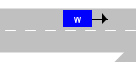
\includegraphics[scale=0.5]{../../concepts/vehicle.png}
        \caption{Vehicle}
        \label{fig:vehicle}
    \end{figure}

    \paragraph{Vehicles}
    Vehicles define the transportation capacities available on the transportation infrastructure.
    Each vehicle must define a maximum battery level, a maximum demand level, a maximum drive speed, and a maximum charge speed, an initial location, and an initial battery level.
    Mathematically, vehicles can be described as elements $v \in V$ with static property functions
    \begin{itemize}
        \item maximum battery level $P_{V.MBL}: V \rightarrow \mathbb{R}^+$,
        \item maximum demand level $P_{V.MDL}: V \rightarrow \mathbb{R}^+$,
        \item maximum drive speed $P_{V.MDS}: V \rightarrow \mathbb{R}^+$,
        \item maximum charge speed $P_{V.MCS}: V \rightarrow \mathbb{R}^+$,
        \item initial location $P_{V.IL}: V \rightarrow L$, and
        \item initial battery level $P_{V.IBL}: V \rightarrow \mathbb{R}_0^+$.
    \end{itemize}
    Furthermore, the dynamic state of vehicles comprises the current location, the current demands, the current demand level, the current charge station, the current battery level, the current drive speed, and the current charge speed.
    Mathematically, the state of vehicles $v$ can be described using dynamic state functions with corresponding simple functional relations
    \begin{itemize}
        \item current demands $S_{V.CD}: V \times \mathbb{T} \rightarrow \mathbb{P}(D)$,
        \item current charge station $S_{V.CCS}: V \times \mathbb{T} \rightarrow CS \cup \{\perp\}$ such that, if the current charge station of the vehicle is not empty, the current vehicles of the charge station include the vehicle, i.e.\ $\forall t \in \mathbb{T}, cs = S_{V.CSS}(v,t): cs \neq \perp \Leftrightarrow v \in S_{CS.CV}(cs,t)$,
        \item current location $S_{V.CL}: V \times \mathbb{T} \rightarrow L$ such that, if the current charge station of the vehicle is not empty, the current vehicle location equals to the location of the charge station, i.e.\ $\forall t \in \mathbb{T}, cs = S_{V.CCS}(v,t): cs \neq \perp \Rightarrow S_{V.CL}(v,t)=P_{CS.L}(cs)$,
        \item current battery level $S_{V.CBL}: V \times \mathbb{T} \rightarrow \mathbb{R}_0^+$ such that the value is smaller than or equal to the maximum battery level of the vehicle, i.e.\ $\forall t \in \mathbb{T}: S_{V.CBL}(v,t) \leq P_{V.MBL}(v)$,
        \item current demand level $S_{V.CDL}: V \times \mathbb{T} \rightarrow \mathbb{R}_0^+$ such that is smaller than or equal to the maximum demand level of the vehicle, i.e.\ $\forall t \in \mathbb{T}: S_{V.CDL}(v,t) \leq P_{V.MDL}(v)$,
        \item current drive speed $S_{V.CDS}: S \times \mathbb{T}$ such that the value is smaller than or equal to the maximum drive speed of the vehicle, i.e.\ $\forall t \in \mathbb{T}: S_{V.CDS}(v,t) \leq P_{V.MDS}(v)$, and
        \item current charge speed $S_{V.CCS}: S \times \mathbb{T}$ such that the value is smaller than or equal to the maximum charge speed of the vehicle, i.e.\ $\forall t \in \mathbb{T}: S_{V.CCS}(v,t) \leq P_{V.MCS}(v)$.
    \end{itemize}

    \begin{figure}[htbp]
        \centering
        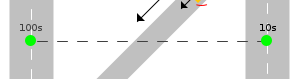
\includegraphics[scale=0.5]{../../concepts/demand.png}
        \caption{Demand}
        \label{fig:demand}
    \end{figure}

    \paragraph{Demands}
    Demands define the transportation loads that temporarily consume the transportation capacities.
    Each demand must define a size, a pick-up location, a drop-off location, an earliest pick-up time, and a latest drop-off time.
    Mathematically, demands can be described as elements $d \in D$ with static property functions
    \begin{itemize}
        \item size $P_{D.S}: D \rightarrow \mathbb{R}^+$,
        \item pick-up location and earliest time $P_{D.PULT}: D \rightarrow LT$ with $P_{D.PULT}(d) = (l_d^{PULT},t_d^{PULT})$, and
        \item drop-off location and latest time $P_{D.DOLT}: D \rightarrow LT$ with $P_{D.DOLT}(d) = (l_d^{DOLT},t_d^{DOLT})$ such that the pick-up location is different from the drop-off location, i.e.\ $l_d^{PULT} \neq l_d^{DOLT}$, and the earliest pick-up time is before the latest drop-off time, i.e.\ $t_d^{PULT} < t_d^{DOLT}$.
    \end{itemize}
    Furthermore, the dynamic state of demands comprises the current vehicle and the current location.
    Mathematically, the state of demands $d$ can be described using dynamic state functions with corresponding simple functional relations
    \begin{itemize}
        \item current vehicle $S_{D.CV}: D \times \mathbb{T} \rightarrow V \cup \{\perp\}$ such that, if the current vehicle of the demand is not empty, the current demands of the vehicle include the demand, i.e.\ $\forall t \in \mathbb{T}, v = S_{D.CV}(d,t): v \neq \perp \Leftrightarrow d \in S_{V.CD}(v,t)$, and
        \item current location $S_{D.CL}: D \times \mathbb{T} \rightarrow L$ such that, if the current vehicle is not empty, the current demand location equals to the current vehicle location, i.e.\ $\forall t \in \mathbb{T}, v = S_{D.CV}(d,t): v \neq \perp \Rightarrow S_{D.CL}(d,t)=S_{V.CL}(v,t)$.
    \end{itemize}

    \subsubsection{Complex functional relations}
    In addition to the simple functional relations some more complex functional relations can be defined over the previous concepts, properties, and states:

    \paragraph{Current charge speed of charge stations}
    The current charge speeds of the charge stations must be derived from the current vehicles of the charge stations and their current charge speeds, i.e.\ $\forall t \in \mathbb{T}, cs \in CS:$
    \[
        S_{CS.CCS}(cs,t)=\sum_{v \in \mathcal{V}}S_{V.CCS}(v,t) \textrm{ with } \mathcal{V}=S_{CS.CV}(cs,t)
    \]

    \paragraph{Current demand level of vehicles}
    The current demand levels of the vehicles must be derived from the current demands of the vehicles and their sizes, i.e.\ $\forall t \in \mathbb{T}, v \in V:$
    \[
        S_{V.CDL}(v,t)=\sum_{d \in \mathcal{D}}^{}P_{D.S}(d) \textrm{ with } \mathcal{D}=S_{V.CD}(v,t)
    \]

    \subsection{State transitions}
    \label{sec:transitions}
    TODO

    \subsection{Discrete events}
    \label{sec:events}
    TODO

    \subsubsection{Vehicle at intersection before}
    TODO

    \begin{figure}[htbp]
        \centering
        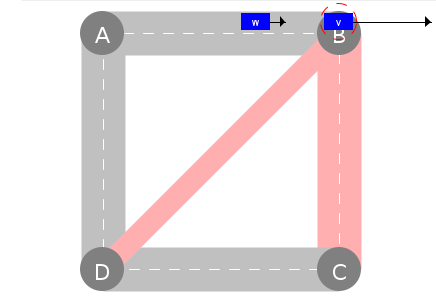
\includegraphics[scale=0.5]{../../events/vehicle-at-intersection-before.png}
        \caption{Vehicle at intersection before}
        \label{fig:vehicle-at-intersection-before}
    \end{figure}

    \subsubsection{Vehicle at intersection after}
    TODO

    \begin{figure}[htbp]
        \centering
        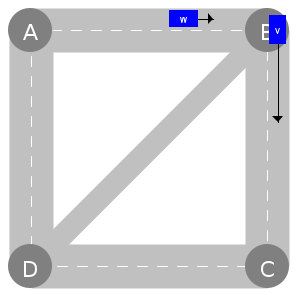
\includegraphics[scale=0.5]{../../events/vehicle-at-intersection-after.png}
        \caption{Vehicle at intersection after}
        \label{fig:vehicle-at-intersection-after}
    \end{figure}

    \subsubsection{Faster vehicle front at slower vehicle back}
    TODO

    \begin{figure}[htbp]
        \centering
        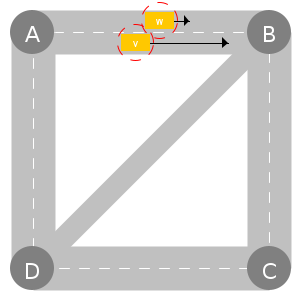
\includegraphics[scale=0.5]{../../events/faster-vehicle-front-at-slower-vehicle-back.png}
        \caption{Faster vehicle f.\ at slower vehicle b.}
        \label{fig:faster-vehicle-front-at-slower-vehicle-back}
    \end{figure}

    \subsubsection{Slower vehicle front at faster vehicle back}
    TODO

    \begin{figure}[htbp]
        \centering
        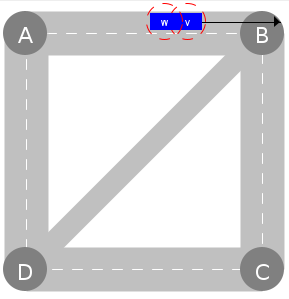
\includegraphics[scale=0.5]{../../events/slower-vehicle-front-at-faster-vehicle-back.png}
        \caption{Slower vehicle f.\ at faster vehicle b.}
        \label{fig:slower-vehicle-front-at-faster-vehicle-back}
    \end{figure}

    \subsubsection{Demand appear}
    TODO

    \begin{figure}[htbp]
        \centering
        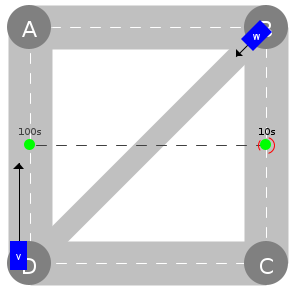
\includegraphics[scale=0.5]{../../events/demand.png}
        \caption{Demand appear}
        \label{fig:demand}
    \end{figure}

    \subsubsection{Vehicle at demand pick-up location}
    TODO

    \begin{figure}[htbp]
        \centering
        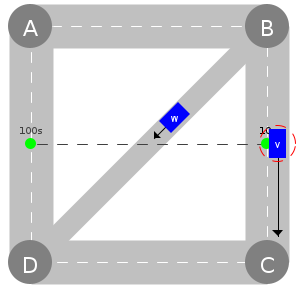
\includegraphics[scale=0.5]{../../events/vehicle-at-demand-pick-up.png}
        \caption{Vehicle at demand pick-up}
        \label{fig:vehicle-at-demand-pick-up}
    \end{figure}

    \subsubsection{Vehicle at demand drop-off location}
    TODO

    \begin{figure}[htbp]
        \centering
        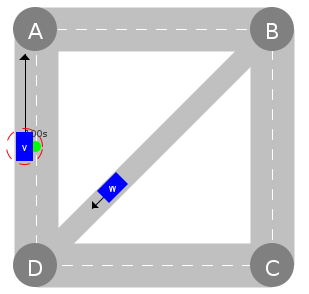
\includegraphics[scale=0.5]{../../events/vehicle-at-demand-drop-off.png}
        \caption{Vehicle at demand drop-off}
        \label{fig:vehicle-at-demand-drop-off}
    \end{figure}

    \subsubsection{Vehicle at station}
    TODO

    \begin{figure}[htbp]
        \centering
        \missingfigure[figwidth=88mm]{Vehicle at station}
        \caption{Vehicle at station}
        \label{fig:vehicle-at-station}
    \end{figure}

    \subsubsection{Vehicle battery full}
    TODO

    \begin{figure}[htbp]
        \centering
        \missingfigure[figwidth=88mm]{Vehicle battery full}
        \caption{Vehicle battery full}
        \label{fig:vehicle-battery-full}
    \end{figure}

    \subsubsection{Vehicle battery empty}
    TODO

    \begin{figure}[htbp]
        \centering
        \missingfigure[figwidth=88mm]{Vehicle battery empty}
        \caption{Vehicle battery empty}
        \label{fig:vehicle-battery-empty}
    \end{figure}

    \subsection{Control interface}
    \label{sec:controller}
    TODO Figure~\ref{fig:controller}

    \begin{figure}[t]
        \centering
        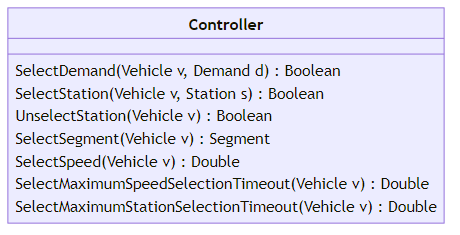
\includegraphics[scale=0.5]{../../diagrams/controller/classes-minimal.png}
        \caption{Controller interface}
        \label{fig:controller}
    \end{figure}

    \subsubsection{Manual controller}
    TODO

    \subsubsection{Random controller}
    TODO
    
    \subsubsection{Greedy controller}
    TODO

    \subsubsection{Smart controller}
    TODO

    \subsection{Statistics interface}
    \label{sec:statistics}
    TODO Figure~\ref{fig:statistics}

    \begin{figure}[htbp]
        \centering
        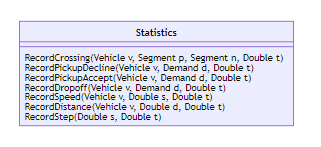
\includegraphics[scale=0.5]{../../diagrams/statistics/classes.png}
        \caption{Statistics interface}
        \label{fig:statistics}
    \end{figure}

    \section{Conclusion}
    \label{sec:con}
    TODO

    \bibliographystyle{plain}
    \bibliography{main}
\end{document}